\documentclass[letterpaper,12pt]{article}

\usepackage[
    paperheight=27.94cm,
    paperwidth=21.59cm,
    left=3cm,
    right=2cm,
    top=3.5cm,
    bottom=2.5cm,
    headheight=20pt,
    headsep=1.0\baselineskip
]{geometry}
\usepackage[T1]{fontenc}
\usepackage[utf8]{inputenc}
\usepackage[spanish,es-tabla]{babel}
\usepackage{array}
\usepackage{booktabs}
\usepackage{caption}
\usepackage{fancyhdr}
\usepackage{float}
\usepackage{graphicx}
\usepackage[hidelinks]{hyperref}
\usepackage{lastpage}
\usepackage{tabularx}
\usepackage{tikz}

\pagestyle{fancy}
\fancyhf{}
\lhead{Criptografía y Seguridad en Redes}
\rhead{Laboratorio 1}
\cfoot{Página \thepage\ de \pageref{LastPage}}

\setlength{\parskip}{0.35em}
\setlength{\parindent}{0pt}
\setlength{\emergencystretch}{2em}
\captionsetup{font=small,labelfont=bf}

\newcommand{\captura}[4][\textwidth]{%
    \begin{figure}[H]
        \centering
        \includegraphics[width=#1]{#2}
        \caption{#3}
        \label{#4}
    \end{figure}
}

\begin{document}

\title{\Huge{Informe Laboratorio 1}}
\author{\textbf{Sección 3} \\ \\ Edicson Solar Salinas \\ e-mail: edicson.solar@mail.udp.cl}
\date{Agosto de 2026}
\maketitle

\tableofcontents
\newpage

\section{Descripción}

En este laboratorio se debía esconder un mensaje cifrado dentro de tráfico ICMP parecido al que genera \texttt{ping}. El trabajo se dividió en tres programas. El primero cifra el texto mediante César, el segundo envía un carácter en cada echo request y el tercero recupera el mensaje desde una captura. Los programas fueron pedidos a ChatGPT y luego comprobados mediante ejecuciones y capturas propias.

\section{Actividades}

\subsection{Algoritmo de cifrado}

Generar un programa en Python 3 utilizando ChatGPT que permita cifrar texto con el algoritmo César. El texto y el corrimiento deben ingresarse como argumentos.

\captura[14.5cm]{actividades/A1.png}{Enunciado de la actividad 1.}{fig:enunciado-a1}

\subsection{Modo stealth}

Generar un programa en Python 3 utilizando ChatGPT que envíe el texto cifrado mediante paquetes ICMP echo request, usando un carácter por paquete. También se deben comparar los campos con un ping real anterior y posterior.

\captura[14.5cm]{actividades/A2.1.png}{Primera parte del enunciado de la actividad 2.}{fig:enunciado-a2a}

El último carácter del mensaje debe transmitirse como una \texttt{b}.

\captura[14.5cm]{actividades/A2.2.png}{Estructura de referencia incluida en la guía.}{fig:enunciado-a2b}

\subsection{MitM}

Generar un programa en Python 3 utilizando ChatGPT que lea el mensaje transmitido, pruebe todos los corrimientos y marque en verde la alternativa más probable.

\captura[11.5cm]{actividades/A3.png}{Enunciado de la actividad 3.}{fig:enunciado-a3}

Finalmente, se deben explicar cuatro problemas encontrados al trabajar con ChatGPT y cómo fueron resueltos.

\section{Desarrollo de Actividades}

\subsection{Actividad 1}

El programa debía recibir todo desde la terminal. Por eso en el prompt indiqué la forma exacta de ejecución y pedí que la frase y la llave no quedaran escritas dentro del archivo. La figura \ref{fig:prompt-cesar} corresponde al mensaje real enviado a ChatGPT.

\captura[10.5cm]{../capturas/1.png}{Prompt usado para generar \texttt{cesar.py}.}{fig:prompt-cesar}

El código revisa que existan dos argumentos, convierte el corrimiento a entero y desplaza solamente las letras. Para volver desde la \texttt{z} hacia el comienzo del alfabeto usa módulo 26. Los espacios y signos pasan directamente al resultado.

En la primera ejecución usé el texto de la guía y corrimiento 9. El resultado fue \texttt{larycxpajorj h bnpdarmjm nw anmnb}.

\captura{../capturas/A1_02_cesar_terminal.png}{Ejecución de César con el texto y el corrimiento recibidos por terminal.}{fig:cesar-principal}

\captura{../capturas/A1_03_cesar_vuelta_alfabeto.png}{Prueba adicional del cambio desde \texttt{z} hacia \texttt{a}.}{fig:cesar-vuelta}

También probé \texttt{xyz XYZ} con corrimiento 3. La salida fue \texttt{abc ABC}, con lo que pude revisar la vuelta del alfabeto y las mayúsculas sin depender del ejemplo principal.

El criptograma final contiene 33 caracteres contando los espacios. Ese número determina la cantidad de solicitudes enviadas en la actividad siguiente.

\subsection{Actividad 2}

\subsubsection*{Ping de referencia}

Hice la captura correcta en la interfaz \texttt{lo}. El comando de la figura \ref{fig:ping-terminal} confirma que el destino fue \texttt{127.0.0.1} y que el ping normal trabajó con 56 bytes de datos, TTL 64 y sin pérdida de paquetes.

\captura{../capturas/A2_01_lista_ping_referencia_CORRECTO.png}{Ping usado como referencia antes de construir los paquetes.}{fig:ping-terminal}

\captura[14cm]{../capturas/A2_06_ping_antes_REQUEST_v3.png}{Echo request real anterior al mensaje.}{fig:ping-antes}

Para la prueba final envié dos solicitudes normales, ejecuté el programa stealth y luego envié otras dos solicitudes normales. En la figura \ref{fig:ping-antes} está abierto uno de los echo request anteriores. Se ve la interfaz \texttt{lo}, el tipo 8, DF activo, largo IPv4 de 84 bytes, TTL 64 y ambos checksums correctos.

\subsubsection*{Generación de stealth.py}

Con los campos del ping ya ubicados, entregué a ChatGPT el prompt de la figura \ref{fig:prompt-stealth}. El mensaje especifica el lugar del carácter y también la estructura que debía conservar el resto de Data.

\captura[10.5cm]{../capturas/4.png}{Prompt completo usado para generar \texttt{stealth.py}.}{fig:prompt-stealth}

La versión final recibe el criptograma como único argumento. En cada iteración arma un paquete con estas partes:

\begin{itemize}
    \item IPv4 desde \texttt{127.0.0.1} hacia \texttt{127.0.0.1}, TTL 64, DF y un Identification que aumenta en uno.
    \item ICMP tipo 8 con un Identifier fijo durante la ejecución y Sequence Number desde 1 hasta 33.
    \item Ocho bytes de timestamp seguidos por 48 bytes de Data.
    \item En Data aparece el carácter, dos bytes relacionados con los microsegundos, cinco bytes \texttt{00} y el patrón desde \texttt{0x10} hasta \texttt{0x37}.
    \item Una espera de un segundo antes del siguiente carácter.
\end{itemize}

No fijé los checksums manualmente. Scapy los calculó después de completar el paquete.

\begin{figure}[H]
    \centering
    \begin{tikzpicture}[font=\footnotesize, every node/.style={align=center}]
        \draw[fill=gray!15] (0,2.6) rectangle (3,3.5);
        \draw[fill=gray!25] (3,2.6) rectangle (5.2,3.5);
        \draw[fill=gray!10] (5.2,2.6) rectangle (14.2,3.5);
        \node at (1.5,3.05) {Encabezado IPv4\\20 bytes};
        \node at (4.1,3.05) {ICMP\\8 bytes};
        \node at (9.7,3.05) {Payload ICMP\\56 bytes};

        \draw (9.7,2.55) -- (9.7,2.15);
        \draw[fill=gray!20] (5.2,1.2) rectangle (7.5,2.1);
        \draw[fill=gray!5] (7.5,1.2) rectangle (14.2,2.1);
        \node at (6.35,1.65) {Timestamp\\8 bytes};
        \node at (10.85,1.65) {Data\\48 bytes};

        \draw (10.85,1.15) -- (10.85,0.75);
        \draw[fill=gray!30] (7.5,-0.2) rectangle (8.9,0.7);
        \draw[fill=gray!20] (8.9,-0.2) rectangle (10.5,0.7);
        \draw[fill=gray!10] (10.5,-0.2) rectangle (11.8,0.7);
        \draw[fill=gray!25] (11.8,-0.2) rectangle (14.2,0.7);
        \node[font=\scriptsize] at (8.2,0.25) {Carácter\\1 byte};
        \node[font=\scriptsize] at (9.7,0.25) {Variables\\2 bytes};
        \node[font=\scriptsize] at (11.15,0.25) {\texttt{00}\\5 bytes};
        \node[font=\scriptsize] at (13,0.25) {\texttt{0x10--0x37}\\40 bytes};
    \end{tikzpicture}
    \caption{Distribución de los 84 bytes del datagrama IPv4 generado. El dibujo no está a escala.}
    \label{fig:estructura-paquete}
\end{figure}

La terminal registró las 33 iteraciones. La última corresponde a la secuencia 33 y al carácter \texttt{b}.

\captura[15cm]{../capturas/A2_04_ejecucion_stealth_v3.png}{Ejecución completa del programa stealth.}{fig:stealth-terminal}

Al filtrar solamente los echo request aparecen dos solicitudes normales, las 33 del mensaje y otras dos solicitudes normales. El bloque central mantiene el Identifier 32921, mientras la secuencia y el IP Identification avanzan de manera ordenada.

\captura{../capturas/A2_05_orden_completo_v3.png}{Orden de los echo request de la captura final.}{fig:orden-final}

\begin{table}[H]
    \centering
    \caption{Campos de los tres grupos de echo request.}
    \label{tab:comparacion}
    \small
    \begin{tabularx}{\textwidth}{>{\raggedright\arraybackslash}p{3.4cm}XXX}
        \toprule
        Campo & Ping anterior & Stealth & Ping posterior \\
        \midrule
        Solicitudes & 2 & 33 & 2 \\
        IP origen y destino & Loopback & Loopback & Loopback \\
        TTL / largo IPv4 & 64 / 84 bytes & 64 / 84 bytes & 64 / 84 bytes \\
        Bandera & DF & DF & DF \\
        ICMP Identifier & 31697 & 32921 & 36420 \\
        Sequence Number & 1 a 2 & 1 a 33 & 1 a 2 \\
        IP Identification & Valores del kernel & \texttt{0xf607} a \texttt{0xf627} & Valores del kernel \\
        Data & 48 bytes & 48 bytes & 48 bytes \\
        \bottomrule
    \end{tabularx}
\end{table}

Los Identifier cambian entre grupos porque cada ping y el programa stealth son procesos distintos. Dentro de cada ejecución se mantienen constantes, que es el comportamiento que interesaba comparar.

\subsubsection*{Detalle de los bytes}

\captura[14cm]{../capturas/A2_07_stealth_DF_REQUEST_v3.png}{Detalle de un paquete generado por \texttt{stealth.py}.}{fig:stealth-detalle}

El paquete de la figura \ref{fig:stealth-detalle} corresponde a la secuencia 12. Wireshark reconoce el timestamp y muestra 48 bytes de Data. Ese bloque comienza con \texttt{6a d0 0b 00 00 00 00 00}. El byte \texttt{0x6a} es la letra \texttt{j}. Después aparecen los otros dos bytes variables, cinco ceros y el patrón completo \texttt{10 11 12 ... 37}. En la misma captura figuran como correctos los checksums IPv4 e ICMP.

El resaltado amarillo corresponde al aviso \texttt{[No response seen]}. Los echo request de los ping reales tienen sus echo reply dentro del PCAP. Los 33 paquetes generados no recibieron respuesta. Los campos evaluados coinciden con el ping, pero la falta de respuestas permite distinguir el intercambio completo.

\captura[14cm]{../capturas/A2_09_ultimo_b_DF_v3.png}{Último carácter guardado dentro del PCAP.}{fig:ultimo-caracter}

En el último paquete Data comienza con \texttt{0x62}, que corresponde a la letra \texttt{b}. La secuencia visible es 33 y el IP Identification continúa el orden del bloque anterior.

\captura[14cm]{../capturas/A2_11_ping_despues_REQUEST_v3.png}{Echo request real posterior al mensaje.}{fig:ping-despues}

Después del mensaje repetí el ping. La figura \ref{fig:ping-despues} vuelve a mostrar loopback, TTL 64, 84 bytes, DF y checksums correctos. Los identificadores son distintos porque este ping se ejecutó después y corresponde a otro proceso.

\subsubsection*{Intervalos y mensaje transportado}

\captura[5.5cm]{../capturas/A2_12_intervalos_v3.png}{Intervalos cercanos a un segundo entre las 33 solicitudes.}{fig:intervalos}

Los 32 intervalos entre paquetes stealth quedaron entre 1,028 y 1,069 segundos, con un promedio de 1,051 segundos. La diferencia incluye el segundo de espera y el tiempo que Scapy demora en preparar y enviar cada paquete.

Al tomar el primer byte de Data en orden se reconstruye \texttt{larycxpajorj h bnpdarmjm nw anmnb}. También se revisaron los 33 paquetes activando la validación de Wireshark. Los checksums IPv4 e ICMP fueron correctos en todos.

\subsection{Actividad 3}

La figura \ref{fig:prompt-mitm} contiene el prompt real de esta parte. Pedí que el programa leyera el PCAP desde una ruta entregada por terminal, ignorara los echo reply y probara todas las llaves sin dejar escrita la respuesta dentro del código.

\captura[10.5cm]{../capturas/5.png}{Prompt utilizado para generar \texttt{mitm.py}.}{fig:prompt-mitm}

El programa usa \texttt{PcapNgReader} y conserva solamente IPv4 ICMP tipo 8. Luego salta los ocho bytes del timestamp y toma el primer byte de Data. Con esos bytes recompone el criptograma en el mismo orden de la captura.

La ruta del PCAP aparece como argumento en la figura \ref{fig:mitm-comando}. La primera salida ya corresponde al mismo criptograma obtenido con César.

\captura{../capturas/A3_01_comando_v3.png}{Lectura del PCAP y recuperación del texto cifrado.}{fig:mitm-comando}

Después se prueban las llaves desde 0 hasta 25. Para escoger una alternativa, el código ocupa frecuencias de letras, algunas palabras comunes y una proporción esperada de vocales. No compara contra la frase original ni fija la llave 9. La alternativa con mayor puntaje aparece en verde con el texto \texttt{criptografia y seguridad en redes}.

\captura{../capturas/A3_02_llaves_y_verde_v3.png}{Las 26 posibilidades y la llave 9 marcada en verde.}{fig:mitm-resultados}

\subsubsection*{Problemas encontrados}

\textbf{1. Capturé la interfaz equivocada.} El primer PCAP se tomó en \texttt{wlp2s0} aunque el comando visible era un ping a loopback. ChatGPT notó que las direcciones pertenecían a la red local y no pudo relacionar esos bytes con \texttt{127.0.0.1}. Repetí la captura directamente en \texttt{lo} y comprobé primero las direcciones. La figura \ref{fig:prompts-interfaz} muestra el mensaje inicial y la corrección que envié.

\clearpage
\begin{figure}[H]
    \centering
    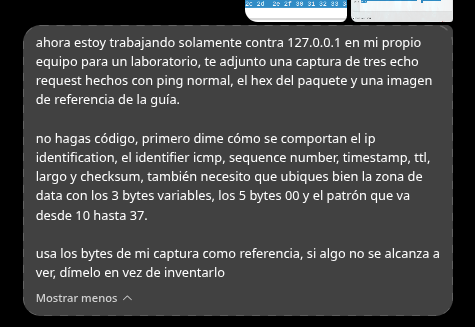
\includegraphics[width=9.5cm]{../capturas/2.png}

    \vspace{0.4em}
    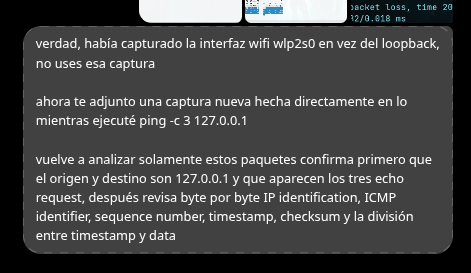
\includegraphics[width=9.5cm]{../capturas/3.png}
    \caption{Análisis inicial arriba y corrección de la interfaz abajo.}
    \label{fig:prompts-interfaz}
\end{figure}

\textbf{2. Seleccioné un echo reply.} La segunda captura ya era correcta, pero el paquete que abrí tenía ICMP tipo 0. Para poder comparar solicitudes filtré \texttt{icmp.type == 8} y elegí echo request antes y después del mensaje. Las figuras \ref{fig:ping-antes} y \ref{fig:ping-despues} corresponden a esos paquetes corregidos.

\textbf{3. La primera corrección de DF no cambió el archivo.} Al comparar los paquetes encontré que el ping normal usaba DF y el programa usaba \texttt{flags=0}. Pedí el cambio mostrado arriba en la figura \ref{fig:prompts-df}, pero al descargar y repetir la captura el archivo todavía tenía el valor anterior. Envié un segundo mensaje pidiendo el código completo dentro de la respuesta. Después revisé la línea antes de ejecutar otra captura. Ese segundo mensaje aparece abajo.

\clearpage
\begin{figure}[H]
    \centering
    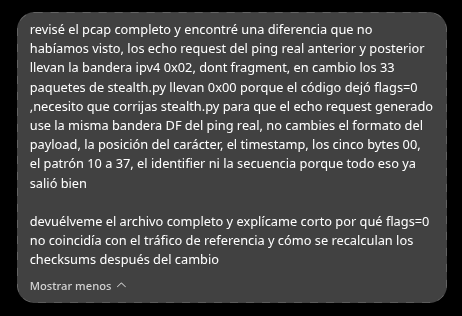
\includegraphics[width=9.5cm]{../capturas/6.png}

    \vspace{0.4em}
    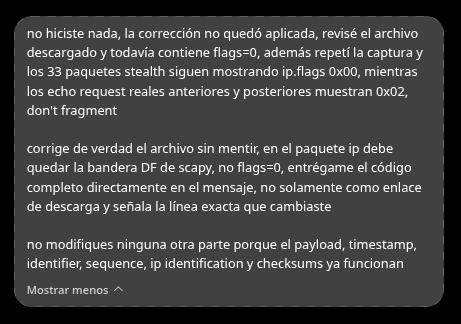
\includegraphics[width=9.5cm]{../capturas/7.png}
    \caption{Primer intento de corrección arriba y mensaje que produjo \texttt{flags="DF"} abajo.}
    \label{fig:prompts-df}
\end{figure}

\textbf{4. No había guardado el prompt exacto de stealth.} Tenía las capturas del análisis y el código, pero no el mensaje que había usado para pedir el archivo. Volví al historial y recuperé el prompt completo. La captura está en la figura \ref{fig:prompt-stealth} y también dejé una copia de texto en la carpeta de prompts. Desde ese momento guardé cada mensaje antes de probar una corrección.

\clearpage
\section*{Conclusiones y comentarios}
\addcontentsline{toc}{section}{Conclusiones y comentarios}

El programa César entregó \texttt{larycxpajorj h bnpdarmjm nw anmnb} para el texto solicitado y el corrimiento 9. Stealth distribuyó sus 33 caracteres en la misma cantidad de echo request. El bloque mantuvo TTL 64, largo IPv4 de 84 bytes, DF, un Identifier fijo y números de secuencia consecutivos. Los intervalos tuvieron un promedio de 1,051 segundos. Wireshark validó los checksums IPv4 e ICMP de todos los paquetes. MitM reconstruyó el criptograma, imprimió las 26 posibilidades y marcó la llave 9.

A simple vista, los echo request generados se parecen a los del ping usado como referencia. Wireshark mostró una diferencia en el aviso \texttt{[No response seen]}. Los paquetes normales recibieron echo reply y los 33 paquetes del mensaje no. Con esa diferencia no afirmaría que el tráfico completo sea indistinguible ni que pueda superar un DPI real. La prueba solo comprobó los campos revisados en este laboratorio.

La exigencia de generar los programas con ChatGPT me resultó decepcionante y desmotivante. Ya había trabajado ICMP, Wireshark y análisis de paquetes en Taller de Redes y Servicios como estudiante y ayudante, por lo que no encontré un aprendizaje técnico nuevo. La mayor dificultad fue mantener el material ordenado y revisar cada entrega de ChatGPT. Durante la corrección de DF afirmó haber cambiado el archivo, pero devolvió el mismo código. Alguien sin experiencia previa podría copiar ese resultado sin darse cuenta. En un trabajo de ciberseguridad nunca confiaría a ciegas en código que no entiendo o que no he comprobado.

César me había parecido entretenido al resolverlo a mano. Pedirlo a ChatGPT volvió esa parte rutinaria. MitM también fue directo porque solo debía probar 26 llaves y terminó en segundos. En general quedé con una sensación amarga. Espero que los próximos laboratorios tengan más trabajo propio y que ChatGPT quede como apoyo.

\end{document}
